\section{长时变化环境下的地图更新}
\label{sec:mapping}
相比于基于稀疏特征的视觉SLAM算法,稠密视觉SLAM技术(dense visual SLAM)通过更注重于维护高质量、可复用的三维地图来帮助传感器定位。由于便携的消费级深度传感器的出现,室内场景的稠密视觉SLAM在近些年取得了不错的进展。KinectFusion~\cite{kinectFusion}首次利用RGBD数据实现了实时的稠密定位和数据融合,并在场景尺度~\cite{voxelHashing}、回环调整~\cite{kintinuous}以及计算效率~\cite{CPUmapping}上有着一系列的拓展。这类方法建立在场景完全静态的严格假设下,当运动物体区域的点云数据被融合到三维地图中,将会带来系统不可逆的崩塌。现有的针对动态场景和环境变化下的定位方法可以分为三类:一类方法只将观测数据中的静态区域融合到三维地图中,确保基于地图的定位方法仍然建立在静态世界的假设下;一类方法分别构建静态地图和动态地图,利用动态地图的历史时序信息作为先验,以提升系统的精度和鲁棒性;还有一类方法维护整个地图在时序上的变化情况,通过引入时间维度的信息将环境描述成一个随时间而转移的状态量,通过反映出的环境变化情况提供更好地预测信息。

\subsection{动态环境下静态部分地图的构建}
\label{subsec:object-centered_mapping}
如前文所述,对于存在运动物体的场景,动态的观测数据违反了基本的几何约束,需要被视为离群点从地图中剔除,这一思想与基于运动分割的SLAM技术十分相似。对于稠密视觉SLAM任务来说,维护静态的三维地图能充分地进行数据融合,也为观测提供了更加完整的运动状态先验。相应地,应对运动物体的挑战主要包括如何避免将运动部分的数据融入地图,如果运动部分数据没有被很好地消除,用于定位的地图信息就会使问题变得复杂起来。

\begin{figure}[thbp]
	\centering
	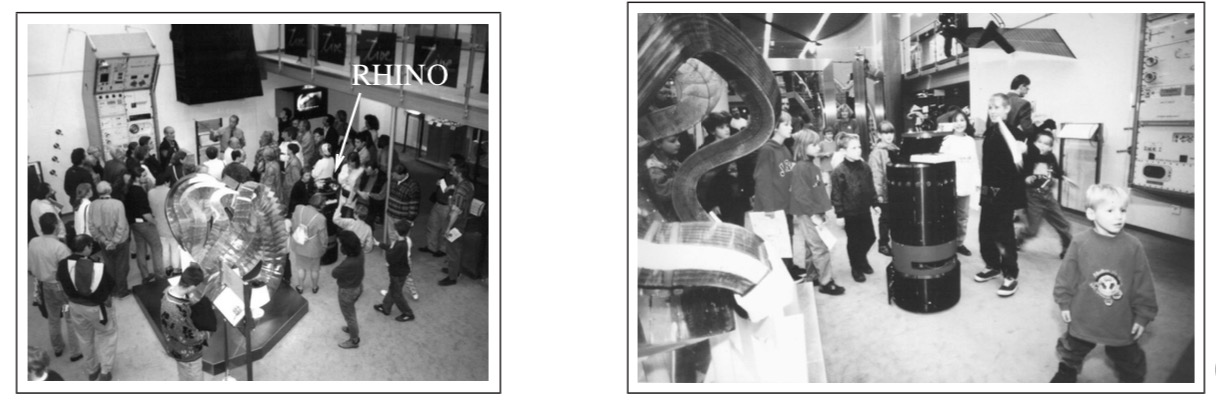
\includegraphics[width=0.9\textwidth]{figs/2-1/early.jpeg}
	\caption{博恩德意志博物馆中的交互式解说机器人Rhino可以在人群中进行准确的自定位~\cite{fox1999}。}
	\label{fig:rhino}
\end{figure}

事实上,通过维护静态地图和采用鲁棒的定位策略在很早的时候就被广泛研究。Fox等人~\cite{fox1999}发现,Markov localization通过维护整个状态空间的概率密度,可以在环境偶尔变化的情况下能够保持稳定,比如门的开关或人的走动。然而,当大量物体没有包含在静态地图中,比如摄像头被室内的人群包围时(如图~\ref{fig:rhino}所示),相机定位将会失败,其主要原因在于马尔科夫假设在高动态环境下并不成立。Fox等人利用entropy filter和distance filter两种滤波方法选出输入数据中没在地图中的部分,将状态空间离散化,从而高效准确地更新置信状态,保证传感器在复杂动态场景下的定位鲁棒性。

ElasticFusion~\cite{elasticFusion}可以应对画面中存在少量运动物体的场景。算法并未显式地检测运动物体,而是将动态环境下的稠密重建作为一个鲁棒估计问题,通过统计的方式自主地将动态区域作为外点剔除。在这个工作的基础上,\cite{keller13_3dv} 从重建的角度出发,认为每个面元只有在多个连续帧被反复观测到才可以融合到三维模型中。当输入的点云数据与匹配上的地图点位置距离过远时,这部分点云会被作为种子点,通过区域生长将当前帧分割成静态和动态区域。相应地,地图上与动态区域有着匹配关系的部分将从地图上剔除掉。通过这种不断更新地图的方式,当之前静态的物体发生运动时,系统可以有效地检测出运动状态的变化,以消除这部分数据对系统鲁棒性的影响。

BaMVO~\cite{BaMVO} 利用背景提取领域(background subtraction)广泛使用的非参数化背景模型进行稠密视觉里程计估计。通过存储连续的4帧深度图并对齐到同一个视角,背景区域可以根据多帧对齐后的深度值差异来进行判别。这样的多帧判别方法建立了时域上的连续性,但是由于采用帧到帧(frame-to-frame)的定位策略,BaMVO不可避免地引入了累计误差。

\begin{figure}[!htbp]
	\centering
	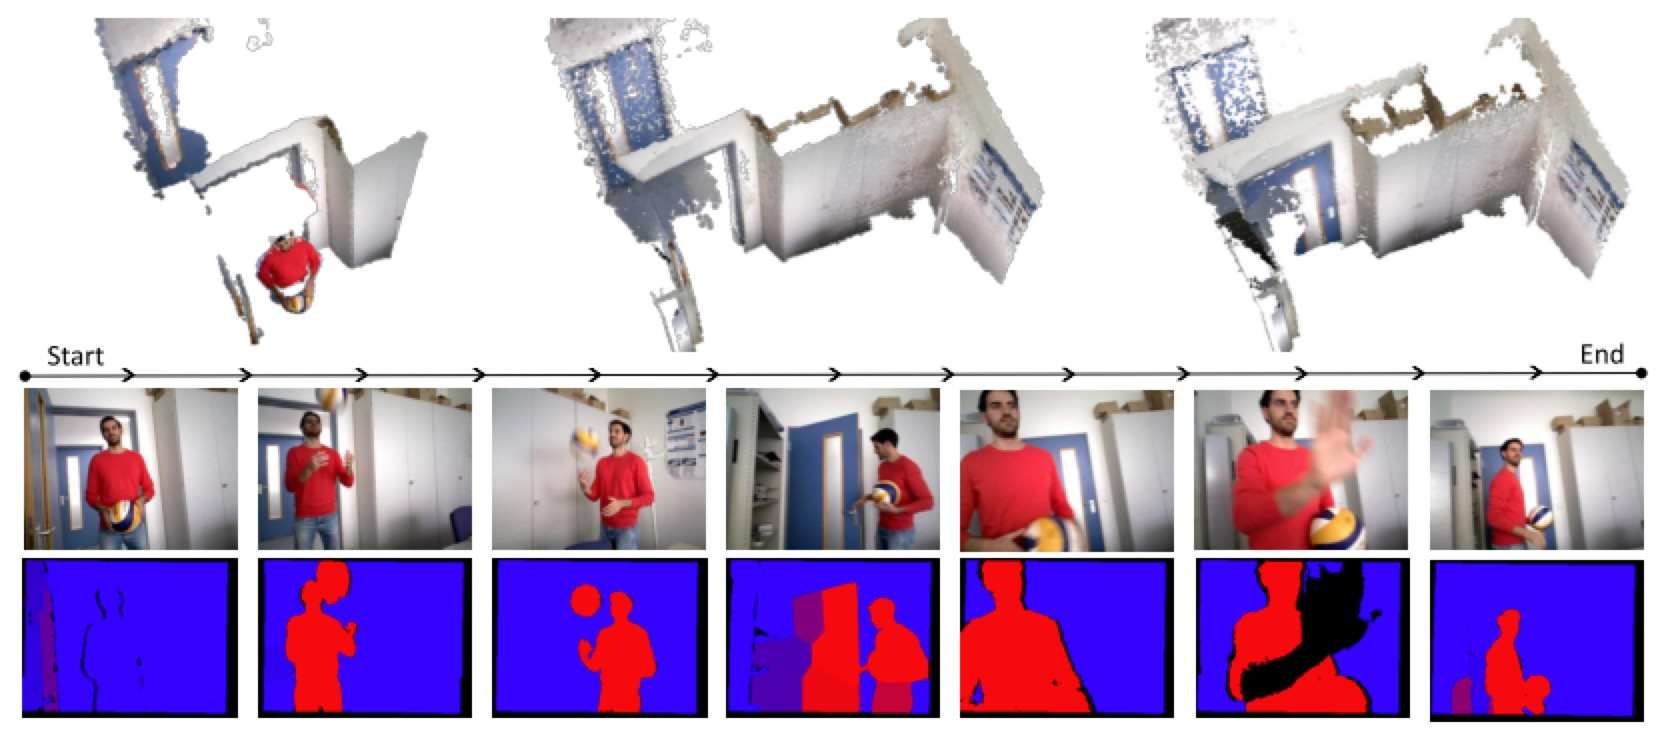
\includegraphics[width=0.9\textwidth]{figs/2-1/staticFusion.jpeg}
	\caption{三维静态地图提供了更加完整的先验,有助于提升运动分割和相机位姿估计这两个子问题的联合求解~\cite{staticFusion}。}
	\label{fig:staticFusion}
\end{figure}

BaMVO说明时序多帧的反馈对动态环境下有效的运动物体检测与分割至关重要,而StaticFusion~\cite{staticFusion}认为有效的时序信息传播可以通过维护一个只包含场景中静态部分的三维地图来实现。三维数据可以有效地进行长时的三维时序信息融合,而数据融合有效地压缩了冗余信息,降低了整个系统的计算代价和内存开销。如图~\ref{fig:staticFusion}所示,通过同时检测运动物体并重建静态环境,staticFusion实现了动态环境下的鲁棒稠密的RGBD SLAM。点云数据被聚类到一个个聚类簇中,每个聚类簇再进行运动状态估计和刚体运动估计的联合求解,以获得每个聚类簇属于静态或动态的概率。被判定为静态的聚类簇内数据会被融合到静态地图中,而被判定动态的聚类簇会进行场景流估计,以实现运动物体时序上的信息传递。由于采用了帧到模型(frame-to-model)的定位策略,相机位姿估计可以有效地消除由于累计误差带来的漂移。

DynaSLAM~\cite{DynaSLAM}提出了一种在线的算法,可以同时在单目、双目和RGBD相机设定下应对环境中的运动物体。整个系统建立在ORB-SLAM~\cite{orbslam2}的前端基础上,而核心出发点是通过建立可复用的三维地图进行更加精确的相机位姿估计。对于单目相机和双目相机,DynaSLAM采用卷积神经网络(CNN)进行像素级的物体分割,作为运动状态估计的先验。在RGBD相机的设定下,由于有着更加可靠的深度信息,DynaSLAM结合了基于稠密地图的几何约束和深度学习的算法进行运动物体检测。如图~\ref{fig:dynaSLAM},通过语义信息与几何约束相结合的方式,DynaSLAM可以应对一些复杂的情形:一类是可能运动的物体在数据采集过程中处于静止状态的情形,比如停着的汽车或者坐着不动的人;另一类是没有运动先验的物体被懂地发生运动的情形,比如人推着椅子行进。这种深度学习与几何相结合的方法可以更好地应对长时复杂多变的环境,在运动状态易变的情况下尽可能地剔除可能发生运动状态变化的数据,建立更稳定可靠的静态地图来帮助定位。

\begin{figure}[!htbp]
	\centering
	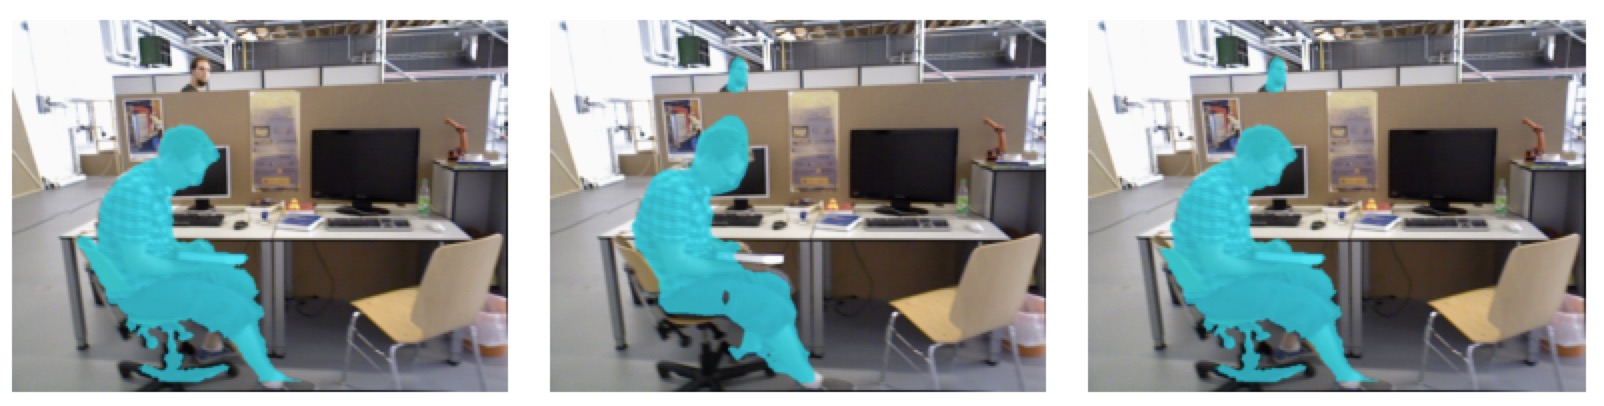
\includegraphics[width=0.9\textwidth]{figs/2-1/dynaSLAM.jpeg}
	\caption{将基于稠密地图的几何约束(左)和基于深度学习的语义信息(中)相结合,可以更好地在复杂的动态环境下进行运动分割(右)~\cite{DynaSLAM}。}
	\label{fig:dynaSLAM}
\end{figure}

当然,在动态环境中构建静态地图依赖静态世界(static world)这一基本假设。在仓库、停车场和住宅这种环境的组成容易发生变化的场景下,环境变化将持续很长的时间,而这种变化可能有利于相机的定位。在极端情形下,可见范围内的静态地图占比很少或者信息量很小的时候,对动态物体运动的推断就对相机位姿估计起到了至关重要的作用。

\subsection{静态背景和动态物体的同时建图}
\label{subsec:static_and_dynamic}
尽管动态物体对于相机位姿的求解会造成干扰,对动态物体的运动估计对于整个系统而言仍然至关重要。一些方法将静态背景与动态物体拆分开来,分别进行三维地图的构建。相比于只维护静态地图的方法,动态物体的运动和几何结构的推断可以带来更好的静态地图和更加可靠的运动分割结果。当然,该类方法的复杂性和计算代价也明显变高,因为算法不仅要通过识别静态背景以获得良好的位姿信息,还需对于每一个运动物体都维护独立的坐标系和地图以进行相应的位姿估计和数据融合。

Meta-room\cite{Ambrus2014Meta}提供了一种杂乱的办公环境的静态建模思路。Meta-room通过迭代地处理点云数据来拆分静态环境,识别环境中的变换元素,并更新地图。发生改变的动态元素将从地图中移除,而之前被遮挡区域会由新的观测数据填充。遮挡问题和传感器噪声在这一框架中需要额外注意。如图\ref{fig:Meta-room-updating}所示,维护一个好的meta-room可以帮助我们找到环境中椅子一类容易频繁移动的物体,构建出meta-object模型,更好地记录下环境随时间的动态变化情况。

\begin{figure}[htbp]
	\centering
	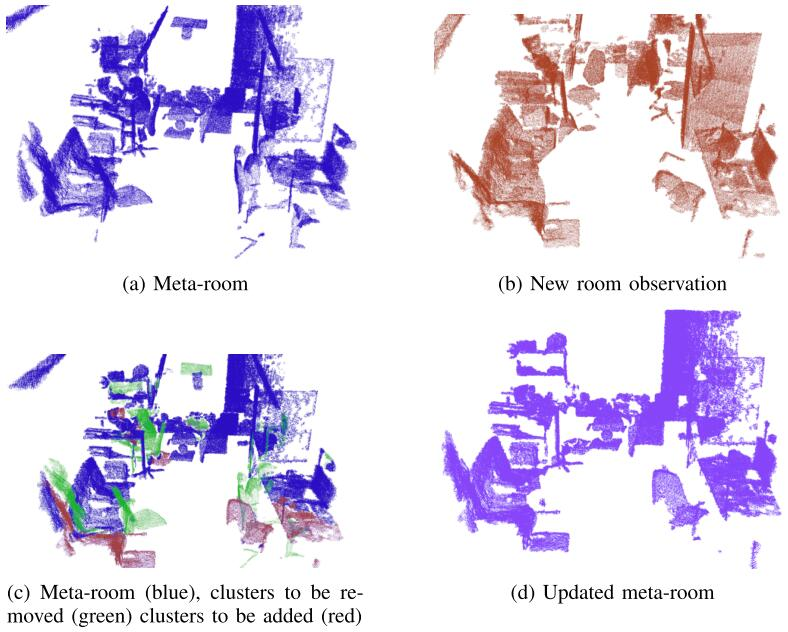
\includegraphics[width=0.75\textwidth]{figs/2-3/meta-room.jpg}
	\caption{meta-room更新过程示意。}
	\label{fig:Meta-room-updating}
\end{figure}

Caccamo等人~\cite{2017Joint3D}使用了自底向上(bottom-up)的特征分类的方式进行物体的识别与分割,如图~\ref{fig:caccamo}所示。算法首先利用第一帧数据初始化静态背景地图,然后将每一帧与静态地图进行配准。运动检测模块将特征分类并将输入数据分到维护的静态地图或物体模型。整个系统建立在基于关键帧的SLAM框架上维护了一个静态的地图,并对输入的每一帧进行特征计算与配准。根据配准之后的误差,将误差较高的部分聚合分离出来,从而判断出与相机运动不一致的动态物体,并维护该动态物体的地图,完成融合。

\begin{figure}[htbp]
	\centering
	\subfloat[]
	{
		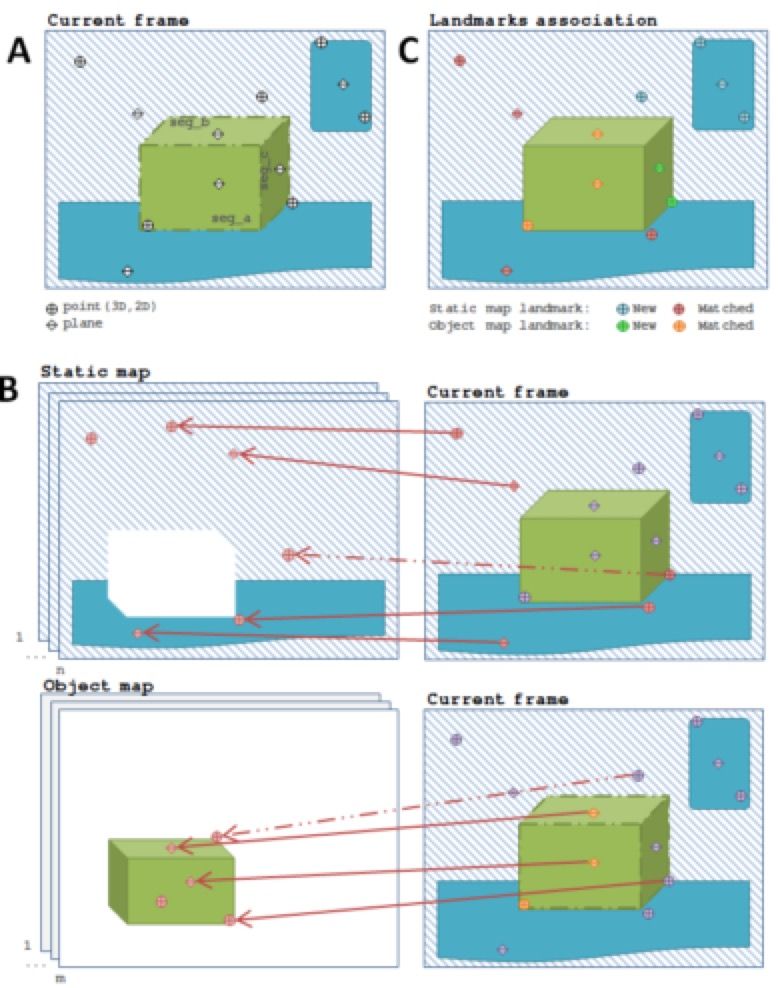
\includegraphics[width=0.25\textwidth]{figs/2-2/caccamo.jpeg} 
		\label{fig:caccamo}
	} 
	\subfloat[]
	{
		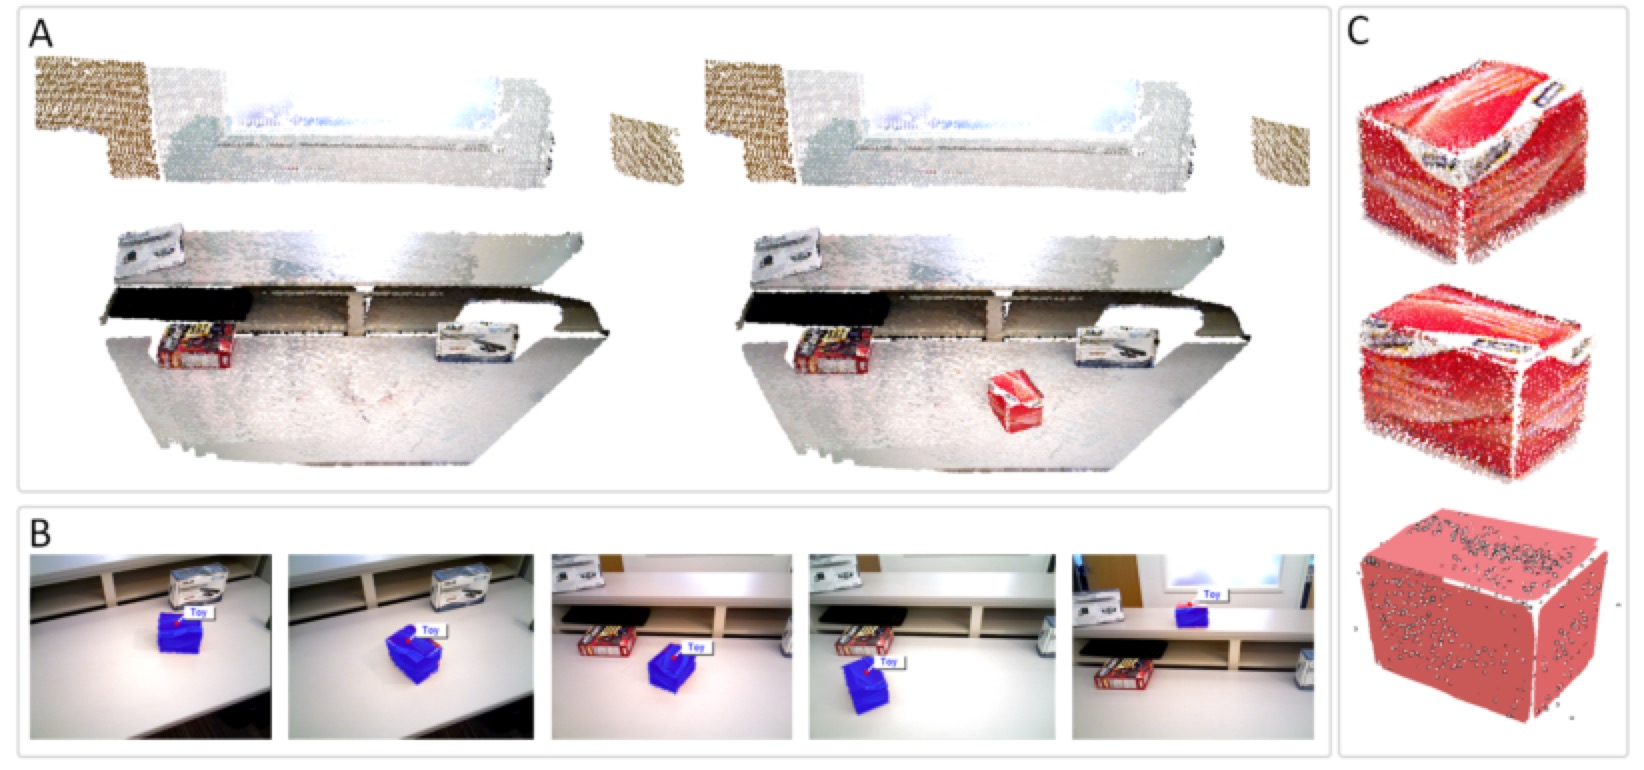
\includegraphics[width=0.65\textwidth]{figs/2-2/caccamo2.jpeg} 
		\label{subfig:caccamo2}
	}
	\caption{(a)观测数据中的平面被组合起来,形成不同的分割区域。基于静态背景的配准可以去除由于运动造成的错误匹配。(b)真实场景下重建得到的完整场景模型。}
	\label{fig:subfigures}
\end{figure}


\begin{figure}[htbp]
	\centering
	\subfloat[MaskFusion算法结构框图]
	{
		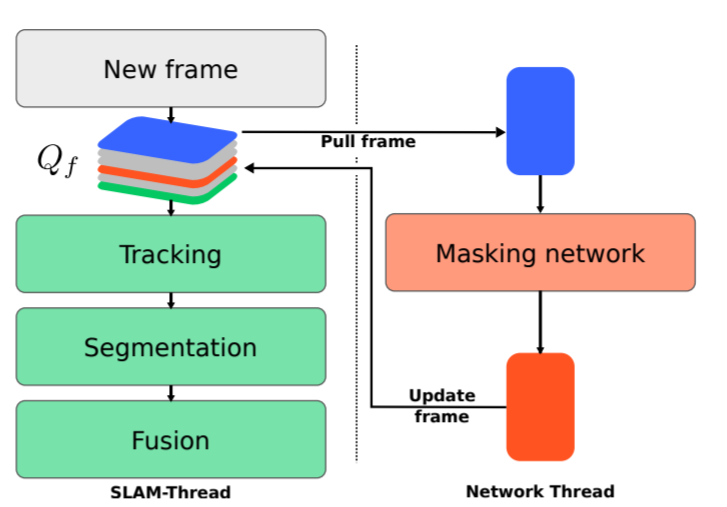
\includegraphics[width=0.45\textwidth]{figs/2-2/maskfusion.png} 
		\label{subfig:MaskFusion-framework}
	} 
	\subfloat[物体分割的各个约束]
	{
		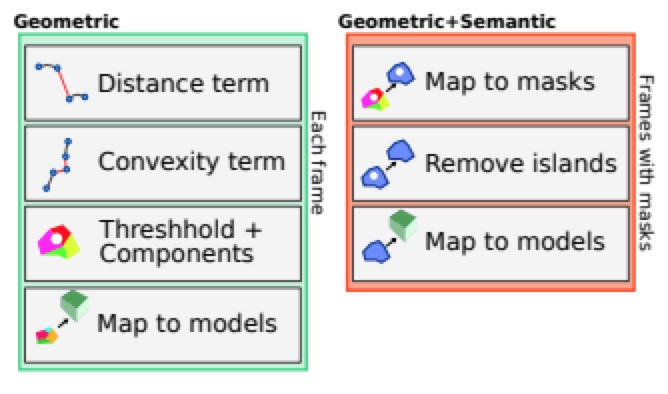
\includegraphics[width=0.45\textwidth]{figs/2-2/maskfusion2.jpeg} 
		\label{subfig:MaskFusion constraint}
	}
	\caption{MaskFusion~\cite{2017MaskRCNN}利用二维图像的语义推断维护了场景中每个物体以及整个静态背景独立的三维模型。}
	\label{fig:subfigures}
\end{figure}

类似的,针对多个物体的同时跟踪与场景模型重建,R\"unz和Agapito~\cite{2017CoFusion}提出了Co-Fusion,可以处理多个不同物体的运动。该方法通过几何约束和语义信息将物体从场景中分割出来,然后对这些物体分别进行跟踪和重建。算法分割出物体后,可对每一部分的三维数据分别进行基于面元的数据融合,以处理不同物体的刚体运动,获得它们的三维模型。这种基于物体分割的动态物体重建会更适用于机器人相关的应用。算法可以对运动的物体获得较为准确的三维信息,从而使得机器人可以与环境进行更为丰富的交互。R\"unz等人之后基于深度学习的方法提出了MaskFusion~\cite{2018MaskFusion},算法将Mask-RCNN~\cite{2017MaskRCNN}的分割结果与形状信息相结合,替代了原有的分割模块,从而在物体的分割边缘上能得到更好的表现,如图~\ref{subfig:MaskFusion-framework}所示。该类方法将语义信息与几何边缘信息相结合,从而获得更加完善的室内场景的物体分割结果。但从另一个角度来说,物体的语义信息依赖于模型的训练集。实验过程中的运动物体需要在训练集中出现过才能得到合理的分割结果,这也是使用语义作为分割标准的一个无法避免的弊端。

\begin{figure}[thbp]
	\centering
	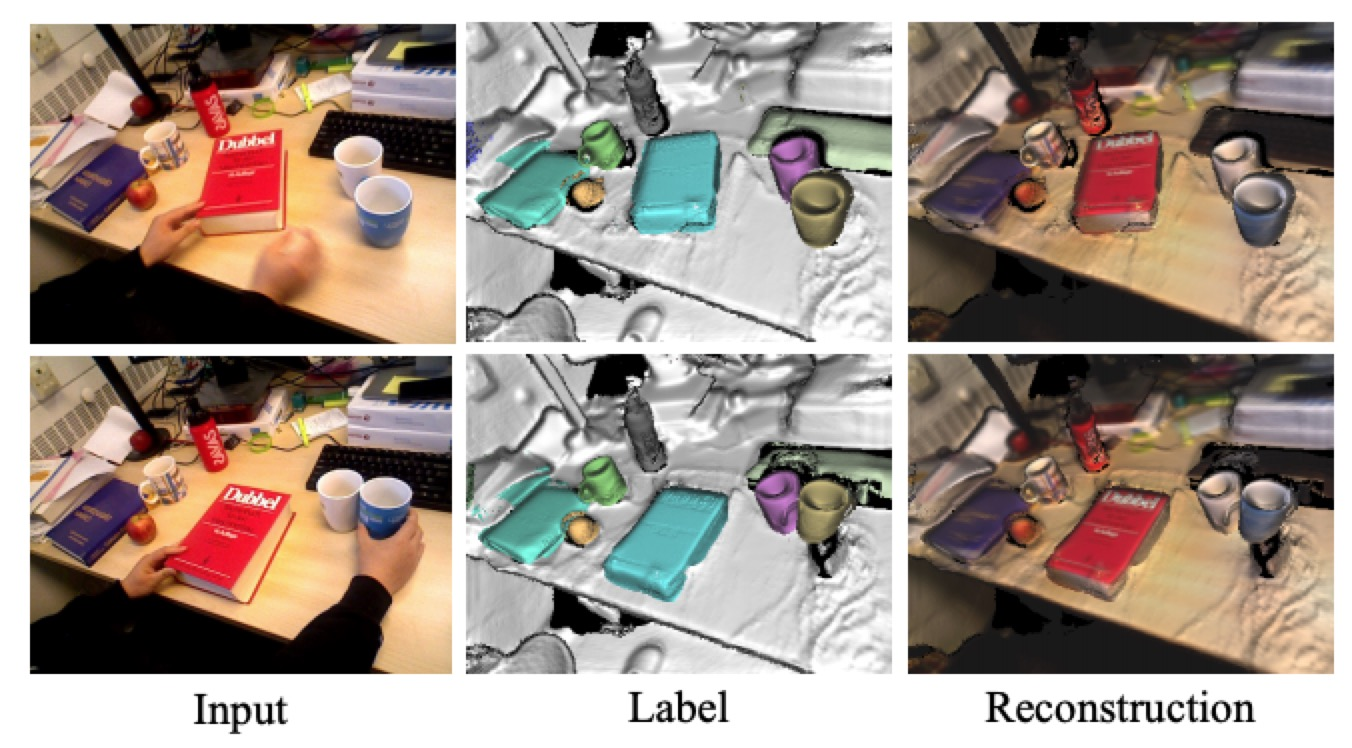
\includegraphics[width=0.9\textwidth]{figs/2-2/midFusion.jpeg} 
	\caption{MidFusion算法~\cite{2019MIDFusion}构建了物体级(object-level)的稠密体素地图,可以应对移动的物体,并忽略场景中人的运动。}
	\label{fig:midFusion}
\end{figure}

相较于使用语义信息进行自顶向下的分割,Xu等人 ~\cite{2019MIDFusion}使用实例分割(instance segmentation),并通过几何和运动信息进行分割结果的优化,获得更好的分割边缘。如图\ref{fig:midFusion}所示,三维地图中不仅仅只维护了几何和颜色信息,也保留了语义类别和运动状态的先验,以便为系统提供更加鲁棒的预测。对于分割后的物体,算法分别对这些物体进行物体姿态的估计、建图以及数据融合。由于维护了基于体素结构的物体级的三维地图,算法对环境变化和未占用空间有着更强的感知能力,在室内场景的移动机器人领域有着更广泛的应用前景。MidFusion采用基于体素空间的截断符号距离函数(TSDF)作为隐式的空间表示方式。通过计算与最近表面的距离作为空间几何的参量,TSDF在未占用区域(free space)和未探索过的区域相比于点云或面元的表示形式有着更加完整的信息。Fehr等人\cite{Fehr2017TSDF}也利用TSDF表示三维空间,对静态地图和运动物体模型进行不断优化。这样的特性是之前基于点云、面元等空间表示形式所不具备的。



\begin{figure}[htbp]
	\centering
	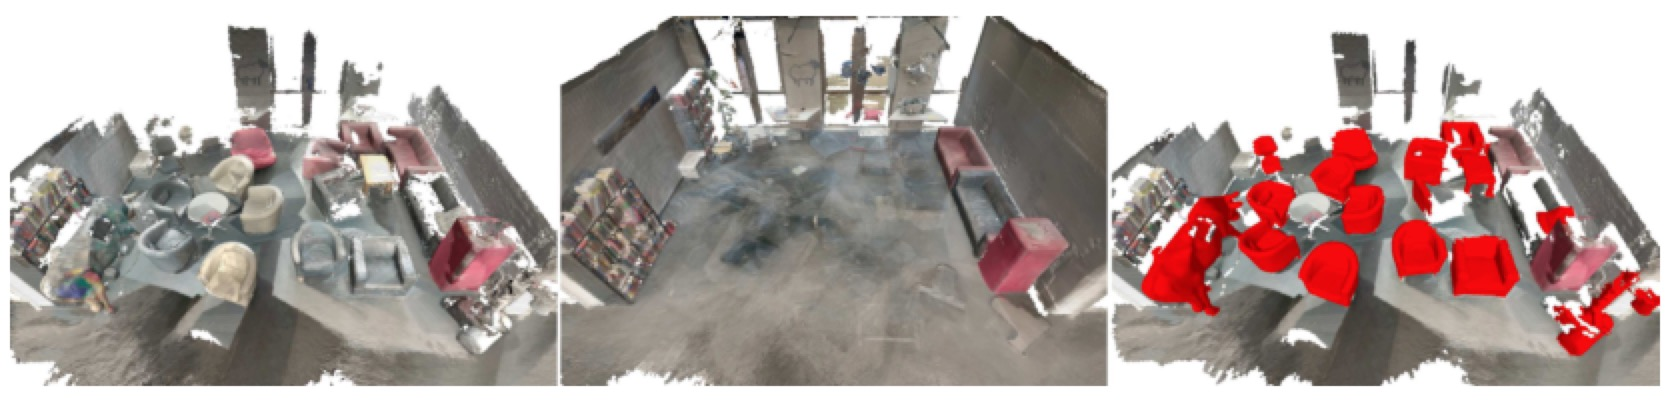
\includegraphics[width=0.9\textwidth]{figs/2-3/tsdf2.jpeg}
	\label{fig:Change-Detection-Overview}
	\caption{基于TSDF的变化检测框架~\cite{Fehr2017TSDF}。}
\end{figure}

\begin{figure}[thbp]
	\centering
	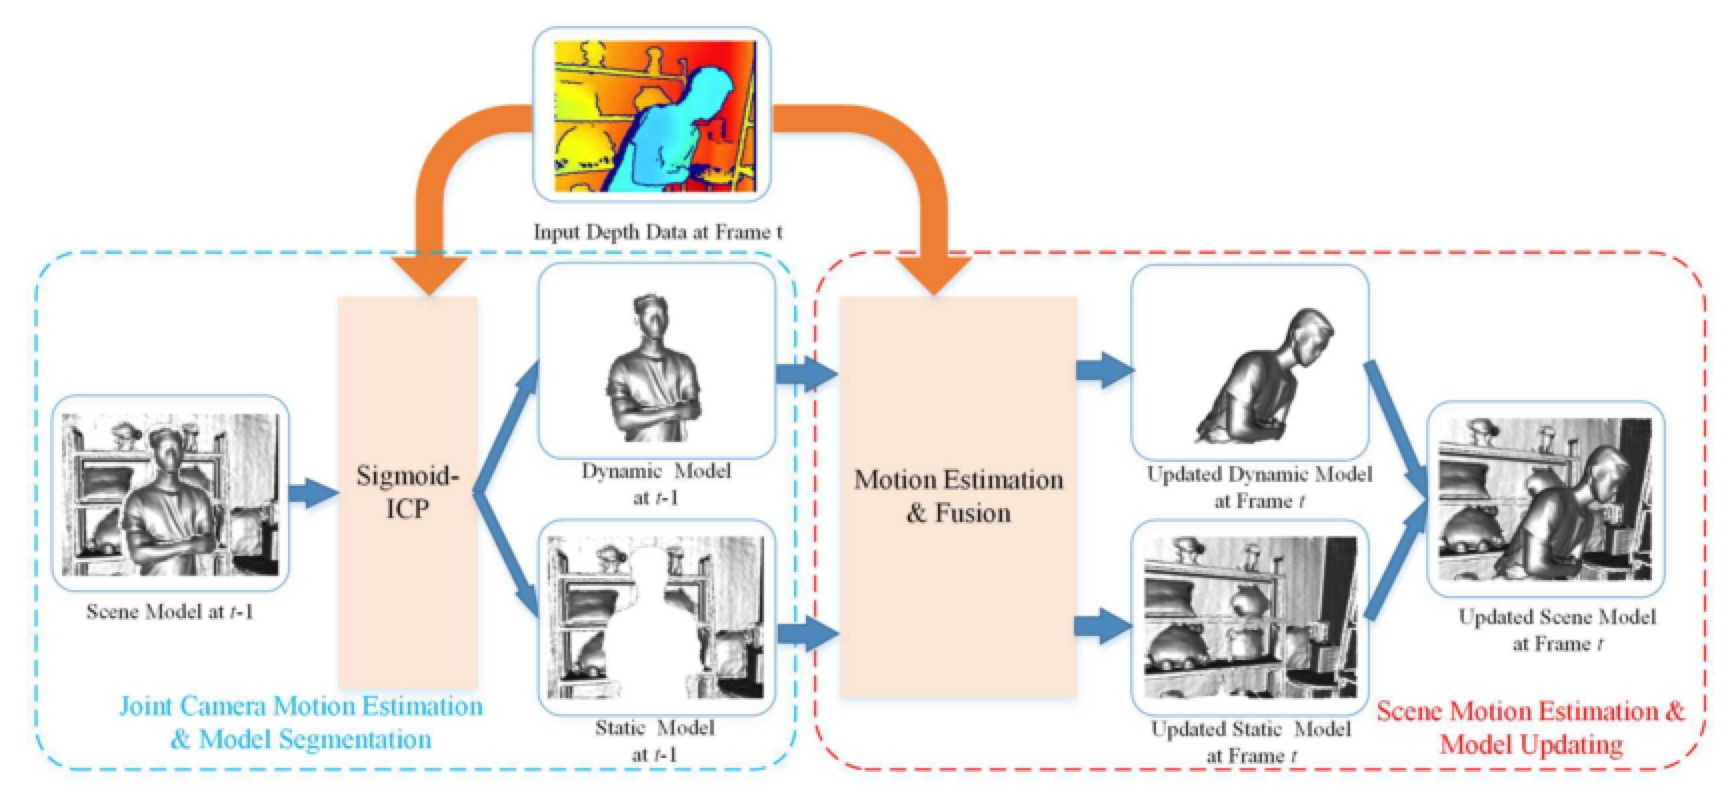
\includegraphics[width=0.9\textwidth]{figs/2-2/mixedFusion.jpeg} 
	\caption{MixedFusion算法~\cite{2017MixedFusion}的流程图。蓝色虚线框内是运动分割和相机位姿估计的联合优化,而红色虚线框内是动态物体运动估计和三维数据融合。}
	\label{fig:mixedFusion-framework}
\end{figure}

相比于前面几种多刚体的环境,MixedFusion~\cite{2017MixedFusion}能够重建出完全非刚体的人体模型。MixedFusion分别维护了每一时刻的运动物体模型和静态背景地图作为整个场景模型,并对输入的每一帧深度信息进行初步配准,区分出静态部分和动态物体。如图~\ref{fig:mixedFusion-framework}所示,场景的静态部分用于相机位姿的估计,而对于动态的部分作者则参考了Newcombe提出的DynamicFusion~\cite{2015DynamicFusion},使用了图节点(graph Node based Motion Representation)将非刚体运动转化为以节点为控制点的多段刚体运动估计。通过运动物体的非刚体运动估计建立当前帧与模板模型(canonical model)的映射关系,来进行动态物体的数据融合。由于mixedFusion只用到了输入的深度信息而丢弃了RGB图像信息,在数据配准时容易受到深度弱纹理的影响,并且难以处理动态物体发生拓扑变化的情况。

总体而言,动态物体与静态场景的同时重建问题是一个较为困难的问题,即便输入为信息最为丰富的RGBD数据,目前也很难给出一个普适性的解决方案,均需要根据情况增加约束以使得问题可解。研究大多着眼于如何区分静态与动态部分,并使用适当的模型来描述动态物体的运动。尽管目前对于单一物体的简单运动可以恢复出较好的模型,但对于多物体复杂运动,考虑到相应的运算开销,常常难以获得较为鲁棒、准确的结果。另一方面,虽然运动部分的输入数据也被保留在地图中,这类方法仍然遵循着静态世界的基本假设,在动态变化较弱的环境下,同时维护静态地图和动态物体模型仍然会和只保留静态地图的方法遇到相似的挑战。

\subsection{四维地图构建与长时定位}
\label{subsec:4Dmapping}
对于动态场景下的地图构建,无论将动态区域作为离群点予以剔除,或是分别维护静态背景和动态物体模型,都依赖于静态世界的假设。为了克服静态世界假设的局限性,一些研究人员致力于在一个统一的表示下建模环境的动态性,并最终达到长时甚至lifelong的建图的目的。早期,Murphy等人~\cite{Murphy1999Bayesian}应用Rao-Blackwellized粒子滤波器(RBPF)来解决SLAM问题,并展示了其在动态场景下的理论可行性。如图\ref{fig:State transition probabilities}所示,他们的方法假设状态转移的概率与环境的当前占据状态独立,并且只能在一个小尺度的局部范围下工作。之后,Avots等人~\cite{Avots2002A}和Petrovskaya等人~\cite{Petrovskaya2007Probabilistic}针对门开合导致的环境变化这一问题对粒子滤波的方案进行了改进:前者用不断维护栅格地图,以得到确切的门的位置;后者则将门的开关状态从是或非的0/1状态改为基于门的打开角度的参数化模型。Stachniss和Burgard~\cite{Stachniss2005Mobile}也使用Rao-Blackwellized粒子滤波器对局部的栅格地图进行聚类,来判断环境中可能存在的物体间的相互关系。Meyer和Delius~\cite{Meyer2010Temporary}维护了一些临时的局部地图,用来跟踪环境中未知的观测数据。传感器的位姿估计则是通过粒子滤波器中维护的全局reference地图和局部地图状态进行估计。然而,这项工作仍然依赖于静态地图进行位姿估计,只有在定位失败时才会利用局部地图。

\begin{figure}[htbp]
	\centering
	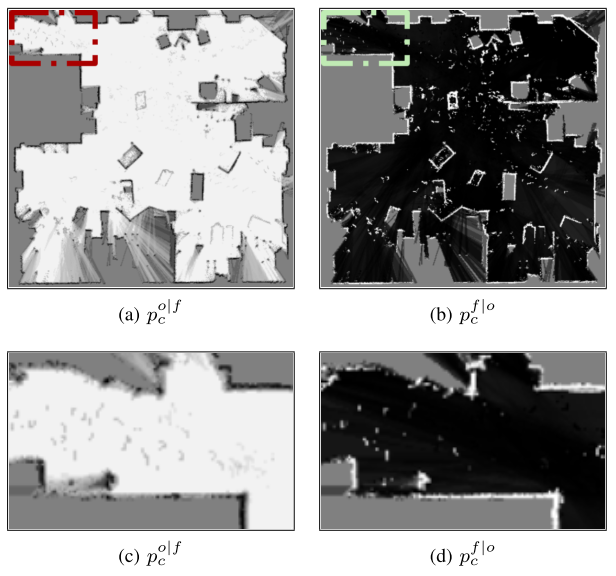
\includegraphics[width=0.6\textwidth]{figs/2-3/filter.png}
	\caption{基于粒子滤波的状态转移概率示意图。(颜色越深,概率越大)。}
	\label{fig:State transition probabilities}
\end{figure}

Churchill和Newman~\cite{Churchill2012Practice}提出了关于lifelong建图的一种新视角。他们认为导航不需要一个全局的地图,而更多地利用拓扑信息。他们利用传感器的已有路径和和对应的观测数据构建了环境的拓扑地图,并称之为“experience”。这种数据驱动的方式可以采用图像匹配进行定位,并通过不断累加的历史路径信息记录环境中experience的变化情况。类似的,Tipaldi等人\cite{Tipaldi2013Lifelong}利用这种拓扑地图的思路改进了已有的粒子滤波的方法,提出了一种新的适应环境变化的lifelong定位方法。它明确地考虑了环境的动态变化,且能够区分:表现出高动态行为的物体,例如汽车和人;可以移动并改变摆放位置的物体,例如箱子、架子或门;以及静止不移动的物体,例如墙壁。该方法在二维占据栅格上用一个隐马尔科夫模型(HMM)描述环境的动态变化,并通过Rao-Blackwellized粒子滤波器高效地迭代更新位姿和地图的状态。

除了基于RBPF的滤波方法,占据栅格也是一种常见的空间表示形式。Chen等人\cite{Chen2006Dynamic}以及后来的Brechtel等人\cite{Brechtel2010Recursive} 提出并拓展了传统的占据栅格(occupancy grid)框架,使之包含了对动态物体的建模,并用贝叶斯滤波的方式对其进行更新,如图\ref{fig: object_tracking_system}所示。在这个视角下,他们认为占据栅格的占据概率由环境中的物体决定。当物体发生运动,其对应的占据栅格也会发生相应的运动。因此,在该框架中,他们需要自始自终追踪每一个栅格的运动。这种从物体出发的建图思路也被成为以物体为中心的环境建模(object-centered reconstruction)。

\begin{figure}[htbp]
	\centering
	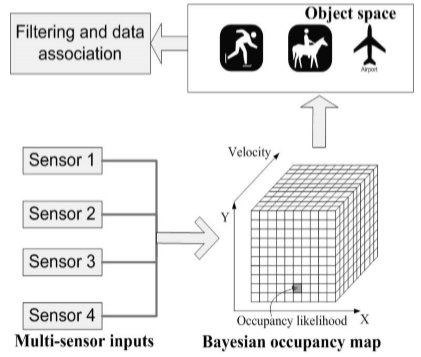
\includegraphics[width=0.4\textwidth]{figs/2-3/bayesian.png}
	\caption{基于贝叶斯滤波器的占据栅格状态更新过程。}
	\label{fig: object_tracking_system}
\end{figure}

为了在lifelong情形下建模变化的环境,Konolige等人~\cite{Konolige2009Towards}提出了一套侧重于地图可视化的框架。在该框架中,局部栅格地图可以随环境的变化进行更新、添加和删减。Kretzschmar等人\cite{Kretzschmar2012Information} 也给出了类似的想法,他们利用一种基于信息论的图修剪策略(graph pruning)进行图压缩操作。这两种方法更侧重于解决长时建图带来的尺度问题。Walcott-Bryant等人\cite{Walcott2012Dynamic}则提出了一个名为Dynamic Pose Graph (DPG)的图模型,针对长时低动态环境进行定位和建图。

与object-centered reconstruction相对应的是从地图角度出发的环境建模(map-centered reconstruction)。这种地图驱动的环境建模方式不过多考虑引起环境变换的原因,而只记录场景在时序上的变化情况。Schindler等人\cite{Schindler2010Probabilistic}自底向上地(bottom-up)地定义了一种时变的场景几何表示方式。在传统的SfM基础上,他们给每个相机加上了对应的时间戳,并为地图中的没一点记录了存在的时间范围。利用概率时序模型,可以从如图\ref{fig: 4D city}建立的“4D城市”几何模型中推断出观测数据对应的确切年份。

\begin{figure}[htbp]
	\centering
	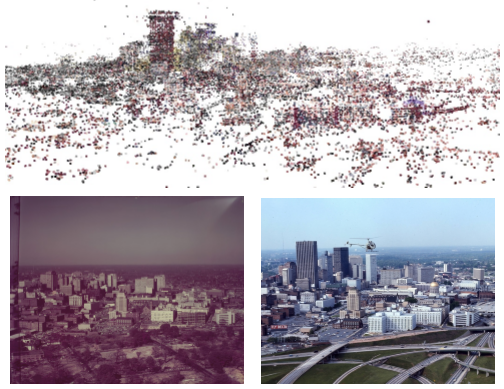
\includegraphics[width=0.6\textwidth]{figs/2-3/city.png}
	\caption{“4D城市”示意图(1956年-1971年)。}
	\label{fig: 4D city}
\end{figure}

%Yang和Wang\cite{Yang2011Feasibility}建议用一个“可能性”网格来同时表示静态区域和动态区域。一对对偶传感器模型被用来在移动机器人定位中判别静态及动态物体,然而,他们的工作假定机器人的位置是已知的,具有一定的精度来进行计算以及更新地图,所以该方法并不适合于全局定位问题。

%\begin{figure}[htbp]
%	\centering
%	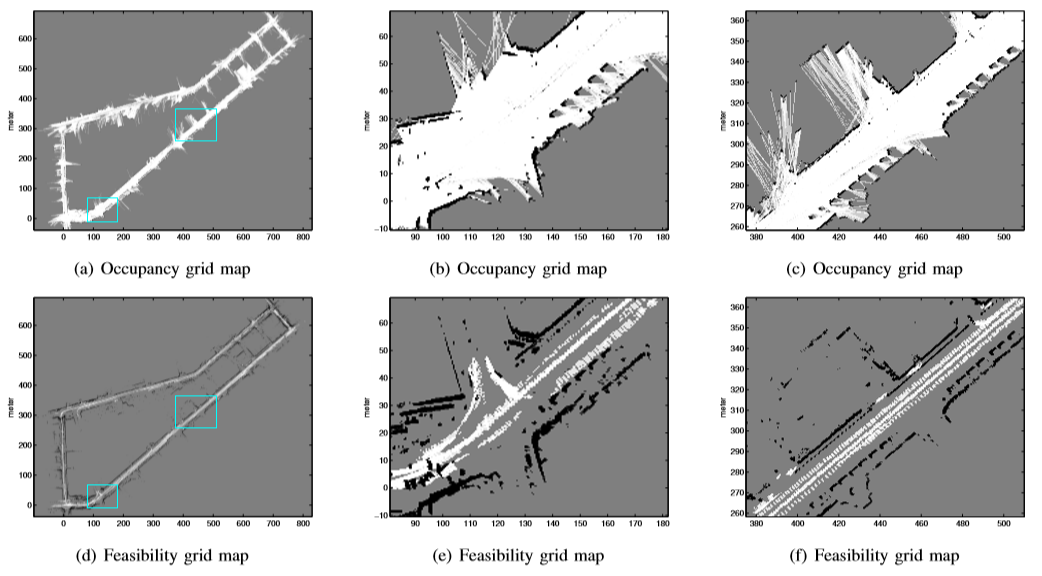
\includegraphics[width=0.9\textwidth]{figs/2-3/feasible.png}
%	\label{fig: Grid maps}
%	\caption{含“可能性”的网格图。}
%\end{figure}

%之后,Saarinen\cite{Saarinen2012Independent}等人提出用一系列独立的马尔科夫链去建模整个环境,将状态之间的转换参数建模为两个泊松过程并在线学习这些参数,采用基于近因加权的方法处理非平稳单元的动力学问题。而同样的,该方法也无法普适地应对真实环境下的不同的动态场景及物体。

\begin{figure}[htbp]
	\centering
	\subfloat[时变的占据栅格示意图(绿色为静态栅格,红色为周期性变化栅格)。]
	{
		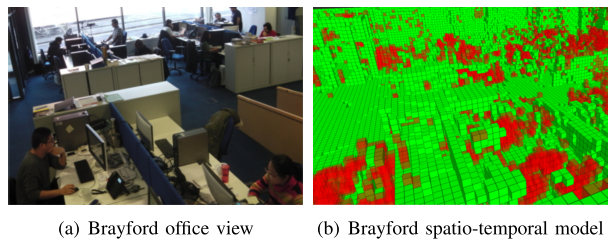
\includegraphics[width=0.5\textwidth]{figs/2-3/spectural3.png} 
		\label{subfig:spectural1}
	} 
	\hspace{1pt}
	\subfloat[时空信息熵随时间和场景动态发生改变。]
	{
		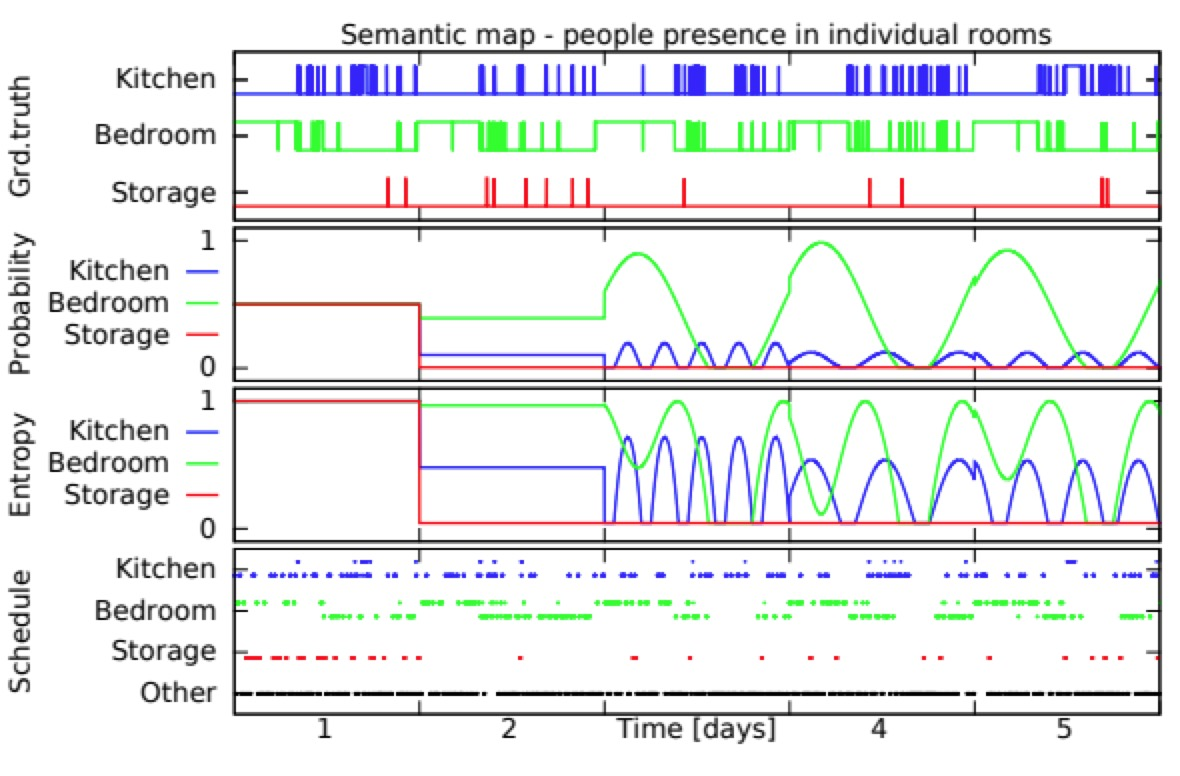
\includegraphics[width=0.4\textwidth]{figs/2-3/spectural4.jpeg} 
		\label{subfig:spectural2}
	}
	\caption{Lifelong设定下移动机器人在变化环境的探索示意\cite{Krajnik2015Life}。}
	\label{fig:subfigures}
\end{figure}

之后,Krajník等人\cite{Krajn2014Spectral}利用频谱建模环境的时空动态信息。这种频谱的空间表示形式可以高效地识别、分析和记忆环境的周期性变化,对于长时的机器人相关应用来说,这种周期性的信息使得模型有着很强的预测能力。文章通过傅里叶逆变换(inverse Fourier transform)来识别长时变化环境下的频谱参数,并用来预测环境的局部状态。傅里叶频谱中最显著的频率组成部分对应着环境中最明显的周期性变化。虽然上述方法适用于移动机器人中使用的大多数环境模型,但由于其依赖于传统的快速傅立叶变换(FFT)方法,因此需要对环境进行定期频繁的观测。这意味着机器人需要首先频繁地访问环境来构建动态模型,然后再利用学习到的动态模型开展导航、路径规划的任务。也就是说,虽然机器人可以创建适合长期操作的动态模型,但它不能在线地维护这些模型。Krajník等人\cite{Krajnik2015Life}在此基础上提出了一种新的思路来解决lifelong设定下移动机器人建模环境的时空变化问题。空间的时空变化模型仍然通过频谱进行表示,而路径规划通过基于信息增益的蒙特卡洛方法实现。机器人利用概率模型和时空信息熵(spatio-temporal entropy)来规划观测,并学习场景的动态变化。该方法增加了一个额外的时间维度,使得机器人不仅可以构建动态模型并不断更新,还可以观察和理解环境自身的变化情况。这种自主智能的环境探索能力能在机器人运动过程中不断优化对环境动态变化的理解。

总而言之,关于如何将静态和动态场景置于一个统一优雅的参数空间下这一问题,研究人员针对时空特性进行了广泛的研究。而在面对实际应用时,基于静态世界假设的三维地图表示仍然是目前的主流技术路线。